\documentclass[12pt]{article}
\usepackage[utf8]{inputenc}
\usepackage[T1]{fontenc}
\usepackage[brazilian]{babel}
\usepackage{graphicx}
\usepackage{amsmath}
\usepackage{hyperref}
\usepackage{geometry}
\usepackage{listings}
\usepackage{xcolor}
\usepackage{subcaption}
\usepackage{minted}

\geometry{margin=1in}

\title{Criacao e Identificacao de Processos em Linux}
\author{Sistemas Operacionais}
\date{\today}

\begin{document}

\maketitle

\section{Introducao}

Este relatorio investiga o comportamento da criacao de processos em Linux, com foco no funcionamento das funcoes \texttt{getpid()}, \texttt{getppid()} e \texttt{fork()}. Foi desenvolvido um programa em C que cria uma hierarquia de processos (pai, filho e neto) com diferentes configuracoes de tempo de espera para observar como o sistema gerencia os identificadores de processos (PIDs) e as relacoes entre processos.

\section{Analise do Programa}

O programa implementa tres experimentos distintos para demonstrar diferentes aspectos do gerenciamento de processos:

\begin{itemize}
    \item \textbf{Experimento A}: "Sem espera" - Nem o filho nem o neto dormem
    \item \textbf{Experimento B}: "Pai espera" - O processo filho dorme por 100 microssegundos
    \item \textbf{Experimento C}: "Neto orfaos" - O processo neto dorme por 100 microssegundos
\end{itemize}

Cada experimento e executado multiplas vezes, e o programa registra o PID e PPID de cada processo em momentos especificos.

\section{Analise dos Resultados}

\begin{figure}[h]
    \centering
    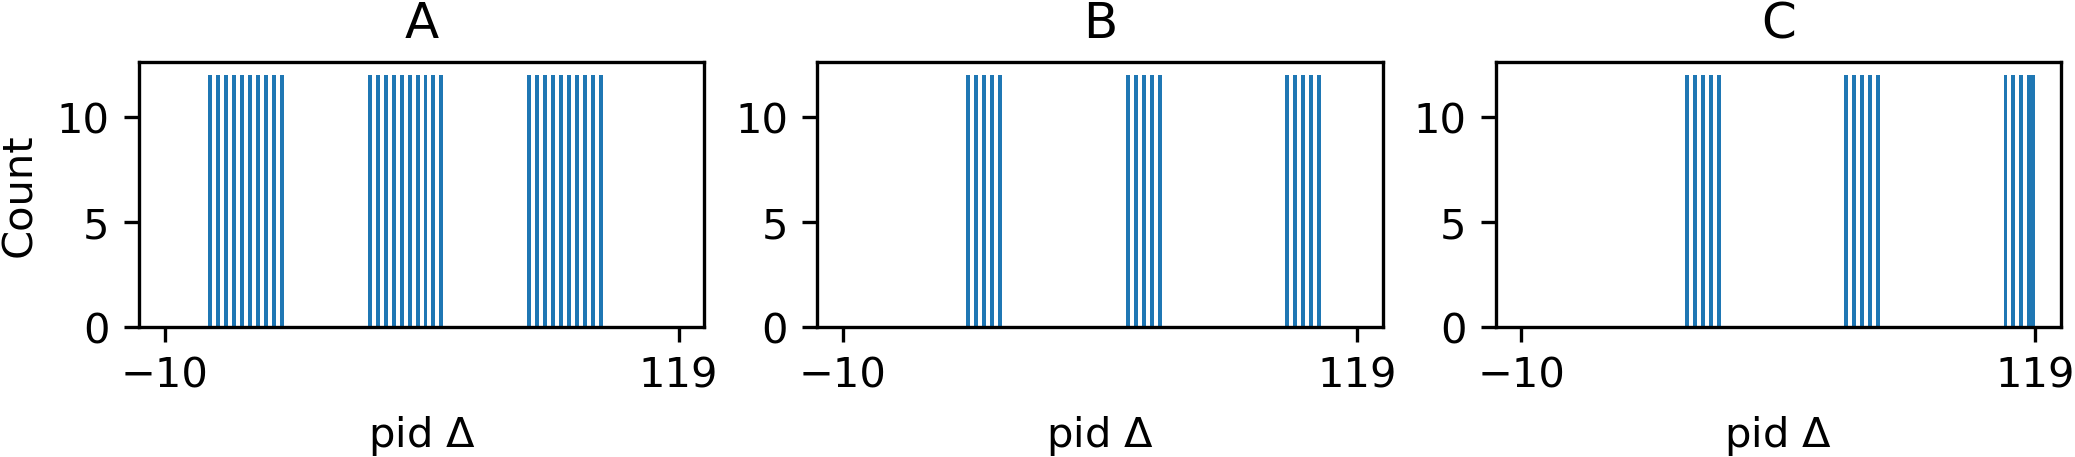
\includegraphics[width=0.8\textwidth]{figures/delta_histogram.png}
    \caption{Histograma da diferenca entre PIDs de processos filhos e seus pais}
    \label{fig:delta_histogram}
\end{figure}

A Figura \ref{fig:delta_histogram} mostra que os PIDs sao atribuidos de forma sequencial, com diferencas pequenas entre processos pai e filho.

\begin{figure}[h]
    \centering
    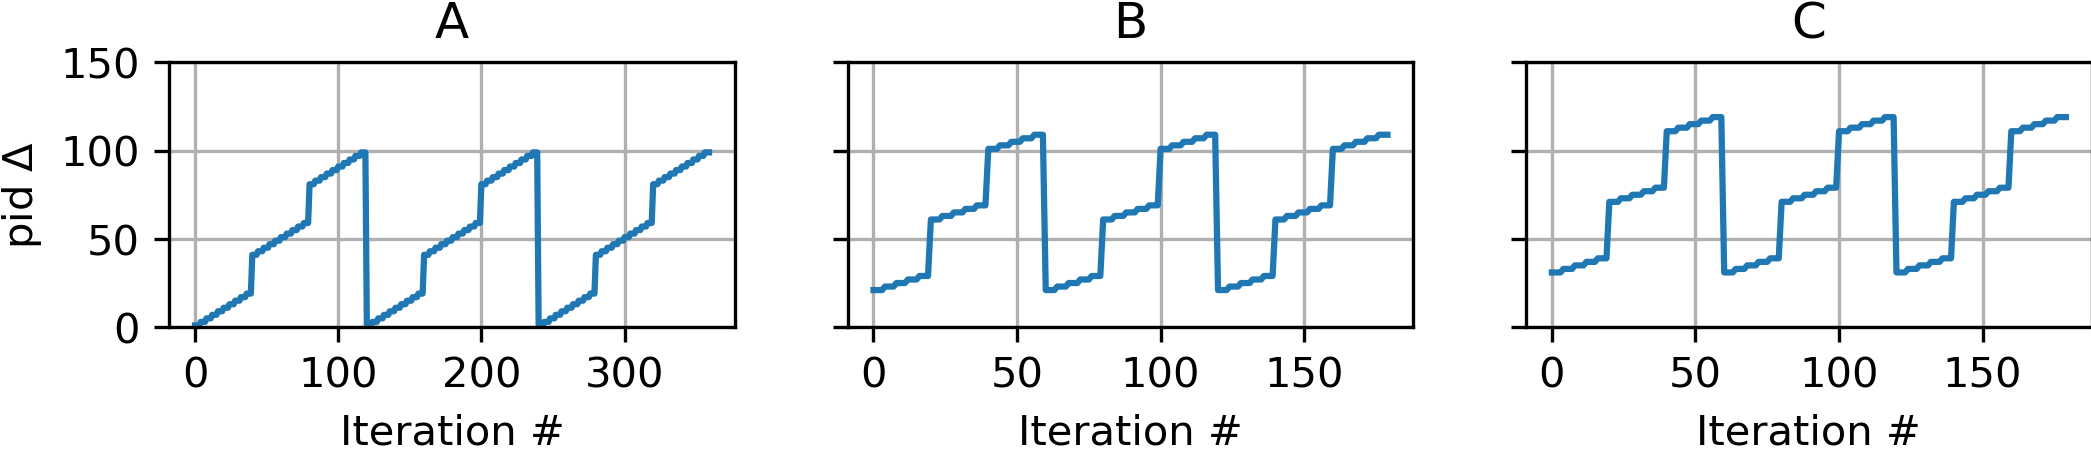
\includegraphics[width=0.8\textwidth]{figures/delta_iteration.png}
    \caption{Variacao da diferenca de PIDs ao longo das iteracoes}
    \label{fig:delta_iteration}
\end{figure}

A Figura \ref{fig:delta_iteration} mostra como a diferenca entre PIDs varia ao longo das iteracoes, confirmando o comportamento sequencial de atribuicao.

\begin{figure}[h]
    \centering
    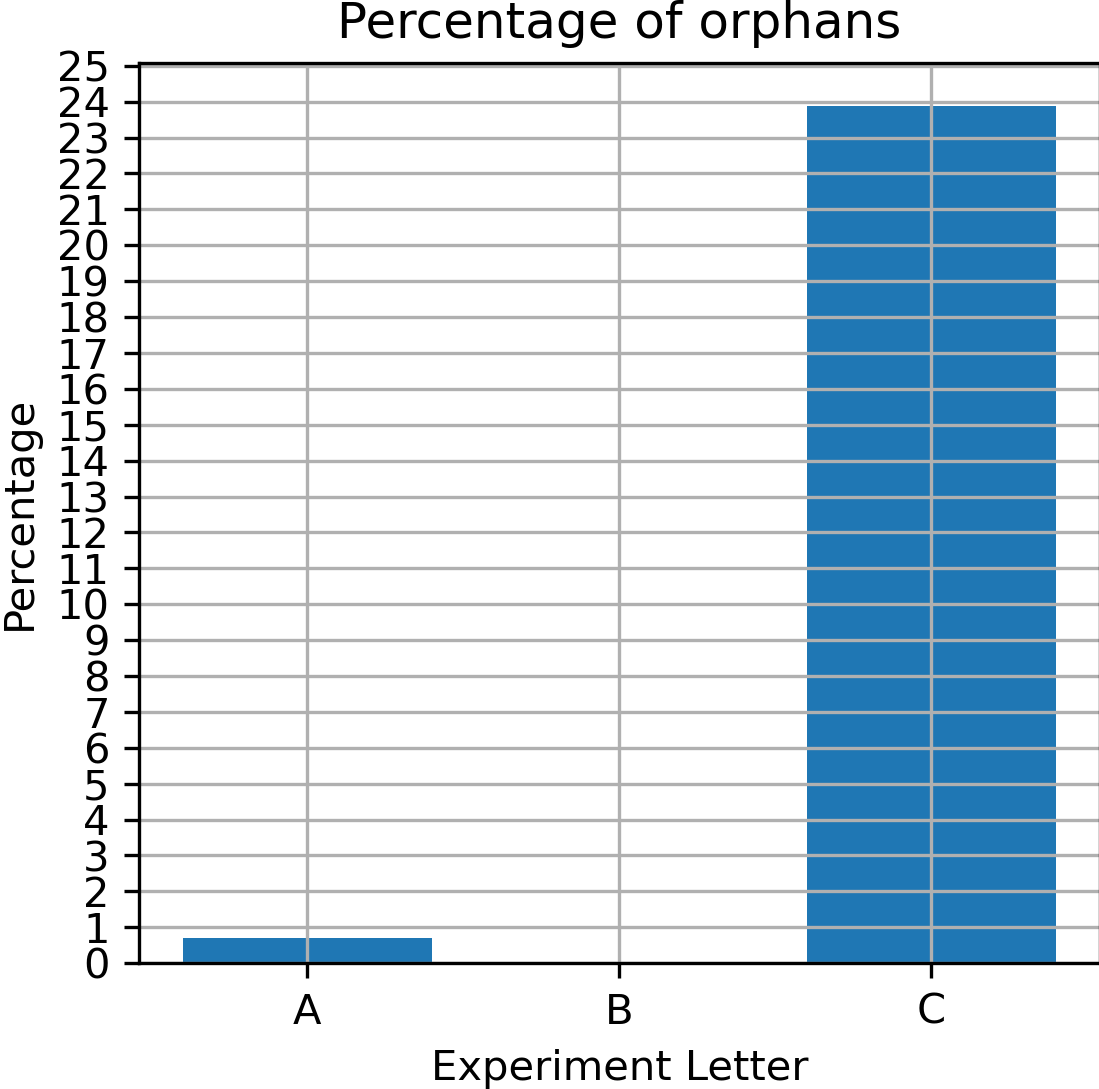
\includegraphics[width=0.5\textwidth]{figures/orphans.png}
    \caption{Porcentagem de processos orfaos por experimento}
    \label{fig:orphans}
\end{figure}

A Figura \ref{fig:orphans} demonstra que no Experimento C, ha mais processos orfaos (com PPID=1) porque o processo filho termina antes do neto acordar, fazendo com que o neto seja "adotado" pelo processo init (PID 1).

\section{Respostas}

\subsection{Diferenca entre getpid() e getppid()}

A funcao \texttt{getpid()} retorna o identificador do proprio processo, enquanto \texttt{getppid()} retorna o identificador do processo pai. O PID e um numero unico para cada processo, e o PPID estabelece a relacao hierarquica entre processos.

\subsection{O que acontece com o PID do processo filho apos o fork()}

Apos o \texttt{fork()}, o filho recebe um novo PID (geralmente o proximo disponivel), enquanto o pai mantem seu PID original. O PPID do filho e configurado como o PID do pai.

\subsection{Como o sistema operacional identifica e organiza os processos}

O Linux usa uma estrutura chamada \texttt{task\_struct} para cada processo, contendo seu PID, PPID, estado e recursos. Os processos sao organizados em arvore hierarquica, onde processos orfaos sao adotados pelo init (PID 1).

\subsection{Previsao do numero de mensagens apos o fork()}

Nao e possivel prever o numero exato de mensagens, pois depende do escalonamento de processos e da temporização entre pai e filho. Com dois \texttt{fork()} em cascata, temos ate quatro fluxos de execucao possiveis.

\subsection{Por que o mesmo programa pode ter multiplos processos com identidades distintas}

Um programa pode ter multiplos processos porque o \texttt{fork()} cria uma copia do processo original com novo PID, permitindo execucao paralela e independente. Cada copia pode seguir caminhos diferentes no codigo, mesmo compartilhando o codigo original.

\section{Conclusao}

Os experimentos demonstram como o Linux gerencia processos, atribuindo PIDs sequencialmente e adotando processos orfaos com o init. Isso e fundamental para a integridade do sistema e para o modelo de concorrencia do Linux.

\section{Apêndice: Código Fonte}

A seguir apresentamos o código-fonte completo do programa utilizado nos experimentos. Este programa cria uma hierarquia de processos pai, filho e neto, com diferentes configurações de tempo de espera para cada experimento.

\subsection{Definições de estruturas e funções auxiliares}

\begin{figure}[ht]
\begin{minted}[frame=lines,fontsize=\footnotesize,linenos,breaklines]{c}
#include <sys/wait.h>
#include <unistd.h>
#include <stdio.h>
#include <stdbool.h>
#include <stdlib.h>
#include <string.h>

struct Experiment {
    size_t repetitions;
    size_t repetition_current;
    char acronym[3];
    char description[40];
    unsigned int sleep_child;
    unsigned int sleep_grandchild;
    pid_t child;
    pid_t grand_child;
};

enum FORK_RESULT {
    FORK_FAIL = -1,
    FORK_CHILD = 0,
    FORK_PARENT = 1,
};

enum FORK_RESULT check_fork(pid_t pid){
    if (pid < 0) return FORK_FAIL;
    if (pid > 0) return FORK_PARENT;
    return FORK_CHILD;
}

void print_process(struct Experiment *e, char const fc[], char id) {
    printf("%s%zu\t%s\t%d\t%d\t%c\n", e->acronym, e->repetition_current, fc,getpid(),getppid(), id);
    setbuf(stdout, NULL);
}

void sleep_process(struct Experiment *e, char const fc[], unsigned int duration){
    printf("%s%zu\t%s\t%d\t%d\tsleep %d\n", e->acronym, e->repetition_current, fc, getpid(), getppid(), duration);
    setbuf(stdout, NULL);
    usleep(duration);
    printf("%s%zu\t%s\t%d\t%d\twokeup\n", e->acronym, e->repetition_current, fc, getpid(), getppid());
    setbuf(stdout, NULL);
}
\end{minted}
\caption{Definições de estruturas e funções auxiliares}
\label{fig:code1}
\end{figure}

\subsection{Função principal de experimento}

\begin{figure}[ht]
\begin{minted}[frame=lines,fontsize=\footnotesize,linenos,breaklines,firstnumber=last]{c}
void experiment(struct Experiment *e) {
    pid_t child_pid = fork();

    e->child = child_pid;
    char fc[2];

    switch (check_fork(child_pid)) {
        case FORK_FAIL:
        break;
        case FORK_CHILD:
            pid_t grand_child_pid = fork();
            e->grand_child = grand_child_pid;
            switch (check_fork(grand_child_pid)) {
                case FORK_FAIL:
                break;
                case FORK_CHILD:
                    strcpy(fc, "G");
                    print_process(e, fc,'A');
                    sleep_process(e, fc, e->sleep_grandchild);
                    print_process(e, fc,'B');

                break;
                case FORK_PARENT:
                    strcpy(fc, "C");
                    print_process(e, fc,'A');
                    sleep_process(e, fc, e->sleep_child);
                    print_process(e, fc,'B');
                break;
            }
            printf("%s%zu\t%s\t0\t0\tE\n", e->acronym, e->repetition_current,fc);
            setbuf(stdout, NULL);

            exit(0);
        break;

        case FORK_PARENT:
            usleep(100 + (e->sleep_grandchild > e->sleep_child ? e->sleep_grandchild : e->sleep_grandchild));
        break;
    }
}
\end{minted}
\caption{Função experiment que implementa a hierarquia de processos}
\label{fig:code2}
\end{figure}

\subsection{Função main}

\begin{figure}[ht]
\begin{minted}[frame=lines,fontsize=\footnotesize,linenos,breaklines,firstnumber=last]{c}
int main() {
    struct Experiment overseer = {3,0,"M\0", "Main\0", 0, 0};

    struct Experiment experiments[] = {
        {10, 0, "A\0", "Experiment A - Sem espera\0", 0, 0}, // sem sono, race
        {5,  0, "B\0", "Experiment B - Pai espera\0", 100, 0}, // filho dorme
        {5,  0, "C\0", "Experiment C - Neto órfãos\0",0, 100}  // neto dorme
    };

    size_t nof_experiments = sizeof(experiments)/sizeof(struct Experiment);

    printf("%s%zu\t%s\t%d\t%d\t%c\n", overseer.acronym, overseer.repetition_current, "I",getpid(),getppid(), 'I');
    setbuf(stdout, NULL);

    for (size_t m = 0; m < overseer.repetitions; m++){
        for (size_t e = 0; e < nof_experiments; e++){
            for (size_t r = 0; r < experiments[e].repetitions; r++ ){
                experiments[e].repetition_current = r;
                experiment(&experiments[e]);
                wait(&experiments[e].child);
                wait(&experiments[e].grand_child);
            }
        }
    }
}
\end{minted}
\caption{Função main que configura e executa os experimentos}
\label{fig:code3}
\end{figure}

\end{document}